\documentclass[11pt,a4paper]{article}

\usepackage[margin=2.4cm]{geometry}
\usepackage{amsmath}
\usepackage{booktabs}
\usepackage{array}
\usepackage{enumitem}
\usepackage{titlesec}
\usepackage{float}
\usepackage{tikz}
\usetikzlibrary{shapes.geometric, arrows.meta, positioning, calc, fit, backgrounds}
\usepackage{hyperref}
\hypersetup{colorlinks=true, linkcolor=black, urlcolor=blue}

% headings: bold, barely larger than the text, well spaced
\titleformat{\section}{\normalfont\large\bfseries}{\thesection.}{0.6em}{}
\titleformat{\subsection}{\normalfont\normalsize\bfseries}{\thesubsection.}{0.6em}{}
\titlespacing*{\section}{0pt}{1.5em}{0.5em}
\titlespacing*{\subsection}{0pt}{1.2em}{0.4em}

\setlength{\parskip}{0.45em}
\setlength{\parindent}{0pt}
\newcommand{\unit}[1]{\,\mathrm{#1}}

% a last-resort stretch so long class names never push past the margin
\setlength{\emergencystretch}{1.2em}

\begin{document}

\begin{center}
  {\large\bfseries How the analyzer reaches its numbers}\\[0.35em]
  {\normalsize From a weight on a scale to the recovery polynomial,
   and what that polynomial is worth}\\[0.9em]
  {\small Suresh Hemal \quad\textbullet\quad 3 October 2026}
\end{center}
\vspace{0.4em}
\hrule
\vspace{1.2em}

{\parskip=0pt
\tableofcontents
}

\vspace{1.2em}

This report answers one question: where do the five coefficients of the recovery polynomial come
from, and what are they worth? It follows a single number all the way through --- from the
weights and lab results in the four CSV files, through the preprocessing that throws runs away
and blanks readings it does not believe, to one run's recovery percentage worked out in full,
to the least squares problem whose solution is those five coefficients, and finally to the
honest answer about how much the fit can be trusted. Along the way it is careful about one thing
that is easy to miss: the five-term equation in real units is not the equation the code prints.
The code logs its inputs, codes them, and chooses its own terms. Both are shown, and the
difference between them is explained rather than glossed over.

\clearpage

\section{The path a number takes}

This section is the map. It follows one number from a cell in a CSV file to a coefficient in
a printed equation, naming the class that does each piece of work. The arithmetic of the
fitting itself comes after; what matters here is the order, and what each stage is allowed
to hand on.

\subsection{Two equations, and which is which}

There are two recovery equations in play and they are not the same equation. Confusing them
is the easiest mistake to make with this project, so they are set out before anything else.

The first is the one asked about:

\begin{equation}
\label{eq:real-units}
\text{recovery \%} \;=\; 33.0192 + 3.16999\,J - 14.4538\,R - 0.0954576\,J^{2}
+ 0.837907\,R^{2}
\end{equation}

Here $J$ is current density in $\mathrm{mA/cm^2}$ and $R$ is the feed ratio in
$\mathrm{mol/mol}$, both in the units the bench reads them in. It is ordinary least squares
over the nine GO-10 runs, with all five estimable terms forced in at once. \textbf{No part of
this project prints equation~\ref{eq:real-units}.} It is a fit made by hand from the nine
rows the analyzer produces, to answer the question ``what do the raw numbers say if you fit
everything''.

The second is what \texttt{uv run limodel analyze} actually prints:

\begin{equation}
\label{eq:coded}
\text{recovery \%} \;=\; 11.5776 - 15.627\,x_2 + 6.08016\,x_2^{2},
\qquad
x_2 = \frac{\ln R - 1.395778}{1.039721}
\end{equation}

Three differences, all of them deliberate and all of them in the code:

\begin{enumerate}[nosep]
  \item \textbf{Logged, coded units.} \texttt{DesignPoints} takes the natural log of each
        setting, then centres and scales it so the runs span $-1$ to $+1$. Equation~\ref{eq:coded}
        is in $x_2$, not $R$.
  \item \textbf{Fewer terms.} \texttt{FittedOutcome} does not fit all five. It grows the model
        one term at a time, keeping a term only if it lowers the leave-one-out error. It kept
        two, and current density never got in at all.
  \item \textbf{No $J$ at all.} Equation~\ref{eq:real-units} has $J$ and $J^2$ with
        coefficients; equation~\ref{eq:coded} has neither, because adding $x_1$ made the
        out-of-sample error worse.
\end{enumerate}

Wherever this report says ``the code's equation'' it means equation~\ref{eq:coded}, and
``the five-term fit'' means equation~\ref{eq:real-units}.

\subsection{The whole pipeline}

Figure~\ref{fig:pipeline} is the shape of the program. \texttt{Analyzer.analyze} is three
lines long and those three lines are the whole order: preprocess, calculate, fit.

Two things are worth noticing in the chart. First, the data changes kind twice. The CSV rows
become \texttt{Run} objects at the loader and stay \texttt{Run} objects through the whole of
preprocessing; they become \texttt{Result} objects at the calculator and are never readings
again. Nothing downstream of \texttt{Calculator} can see a tank weight.

Second, the \texttt{Journal} sits to the side and every stage writes into it. It is one
record, made empty, handed to the \texttt{Analyzer}, and handed on down. Nothing in it
prints as it is written; the \texttt{Analyze} command reads the whole of it at the end. That
is why the report can open with everything that was left out before it shows a single result.

\begin{figure}[htbp]
\centering
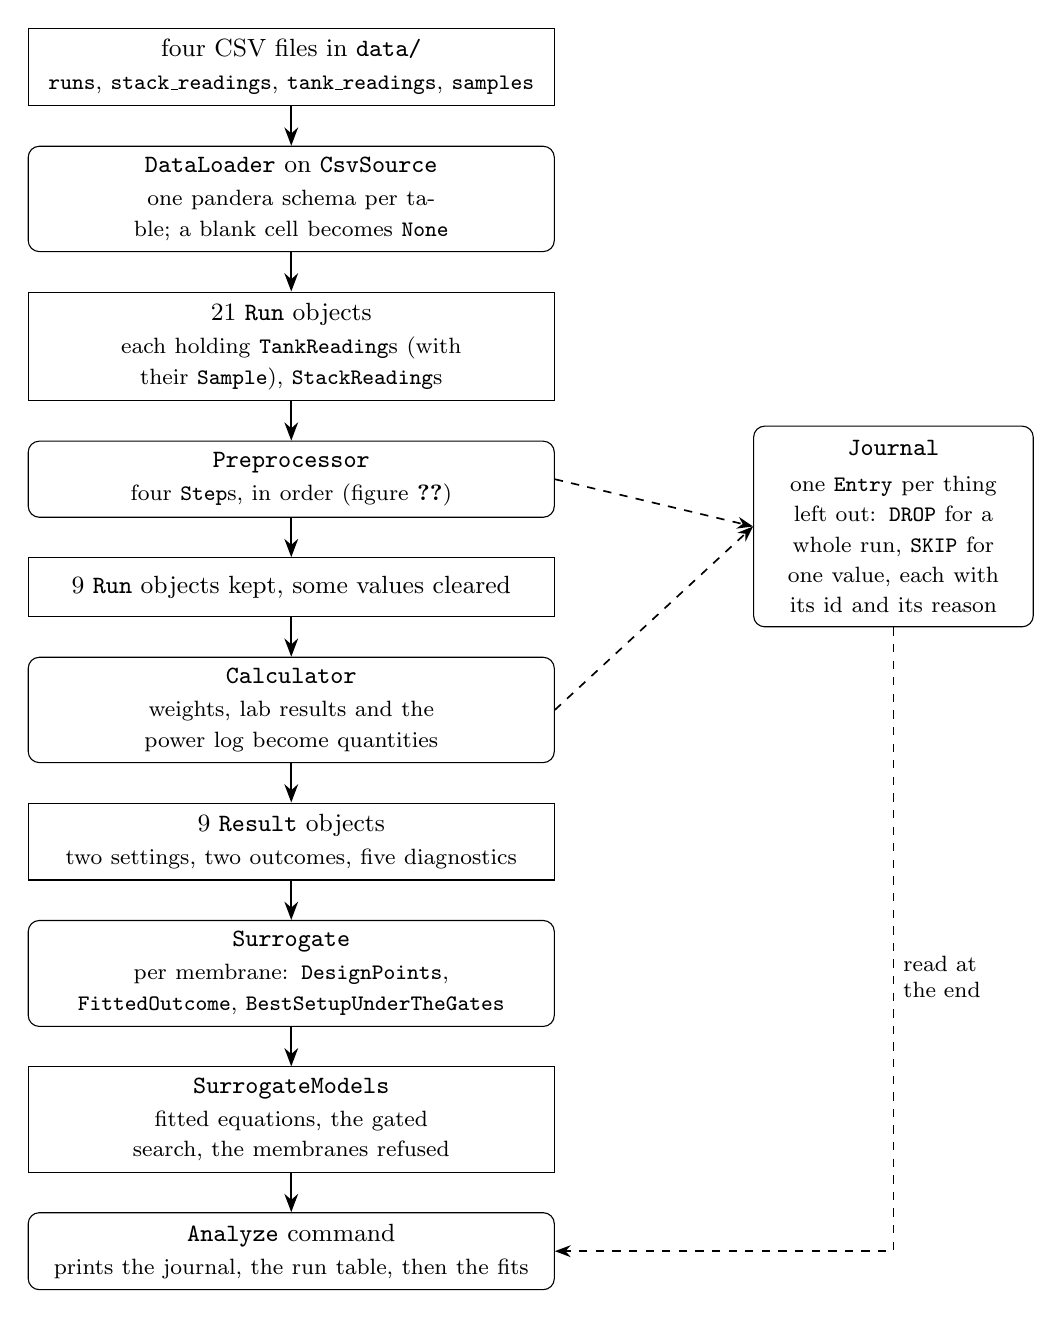
\begin{tikzpicture}[
  node distance=5mm,
  stage/.style={draw, rounded corners, align=center, font=\small, text width=6.4cm,
                inner sep=4pt, minimum height=7.5mm},
  payload/.style={draw, align=center, font=\small, text width=6.4cm,
                  inner sep=4pt, minimum height=7.5mm},
  record/.style={draw, rounded corners, align=center, font=\small, text width=3.2cm,
                 inner sep=5pt},
  flow/.style={-Stealth, thick},
  note/.style={-Stealth, dashed, semithick}
]

\node[payload] (csv)
  {four CSV files in \texttt{data/}\\[1pt]
   \footnotesize \texttt{runs}, \texttt{stack\_readings}, \texttt{tank\_readings},
   \texttt{samples}};

\node[stage, below=of csv] (loader)
  {\texttt{DataLoader} on \texttt{CsvSource}\\[1pt]
   \footnotesize one pandera schema per table; a blank cell becomes \texttt{None}};

\node[payload, below=of loader] (runs)
  {21 \texttt{Run} objects\\[1pt]
   \footnotesize each holding \texttt{TankReading}s (with their \texttt{Sample}),
   \texttt{StackReading}s};

\node[stage, below=of runs] (prep)
  {\texttt{Preprocessor}\\[1pt]
   \footnotesize four \texttt{Step}s, in order (figure~\ref{fig:steps})};

\node[payload, below=of prep] (kept)
  {9 \texttt{Run} objects kept, some values cleared};

\node[stage, below=of kept] (calc)
  {\texttt{Calculator}\\[1pt]
   \footnotesize weights, lab results and the power log become quantities};

\node[payload, below=of calc] (results)
  {9 \texttt{Result} objects\\[1pt]
   \footnotesize two settings, two outcomes, five diagnostics};

\node[stage, below=of results] (surr)
  {\texttt{Surrogate}\\[1pt]
   \footnotesize per membrane: \texttt{DesignPoints}, \texttt{FittedOutcome},
   \texttt{BestSetupUnderTheGates}};

\node[payload, below=of surr] (models)
  {\texttt{SurrogateModels}\\[1pt]
   \footnotesize fitted equations, the gated search, the membranes refused};

\node[stage, below=of models] (cmd)
  {\texttt{Analyze} command\\[1pt]
   \footnotesize prints the journal, the run table, then the fits};

\foreach \a/\b in {csv/loader, loader/runs, runs/prep, prep/kept, kept/calc,
                   calc/results, results/surr, surr/models, models/cmd}
  \draw[flow] (\a) -- (\b);

\node[record] at ($(prep.east)+(4.3,-0.6)$) (journal)
  {\texttt{Journal}\\[2pt]
   \footnotesize one \texttt{Entry} per thing left out: \texttt{DROP} for a whole run,
   \texttt{SKIP} for one value, each with its id and its reason};

\draw[note] (prep.east) -- (journal.west);
\draw[note] (calc.east) -- (journal.west);
\draw[note] (journal.south) |- (cmd.east)
  node[pos=0.28, right, font=\footnotesize, align=left] {read at\\the end};

\end{tikzpicture}
\caption{The pipeline, from four CSV files to a printed equation. Solid arrows carry the
data; the dashed arrows into the journal are writes, and the one dashed arrow out of it is
the command reading the whole record at the end. Rounded boxes do work, square boxes are
what they hand on. The order is
\texttt{Analyzer.analyze}.}
\label{fig:pipeline}
\end{figure}

\subsection{The four preprocessing steps}

\texttt{Preprocessor} holds the four steps as a tuple and runs each on what the one before
returned. Figure~\ref{fig:steps} shows them with the counts on the real data.

The order is a decision. Dropping by membrane comes second so that the reading checks never
spend effort on a run the modelling throws away anyway. Dropping runs the lab cannot answer
for comes \emph{last}, after the checks, so that a run on its way out is still looked over
and its bad readings still get written down: the journal is a record of the whole dataset,
not only of the part that survived.

Two steps drop whole runs and refuse to return nothing: if every run fails,
\texttt{DropExcludedRuns} and \texttt{DropRunsOnAnotherMembrane} both raise rather than hand
on an empty list, because modelling nothing in silence would hide a misspelled membrane
name.

\begin{figure}[htbp]
\centering
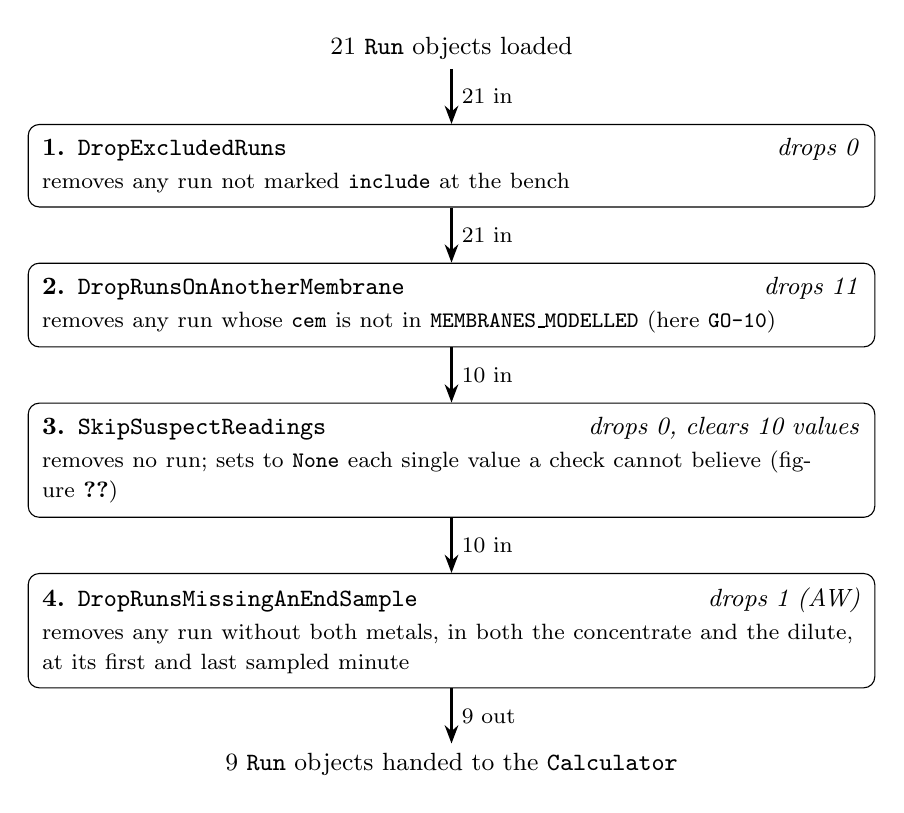
\begin{tikzpicture}[
  node distance=7mm,
  stepbox/.style={draw, rounded corners, align=left, font=\small, text width=10.4cm,
               inner sep=5pt},
  tally/.style={font=\small},
  flow/.style={-Stealth, thick}
]

\node[tally] (in) {21 \texttt{Run} objects loaded};

\node[stepbox, below=of in] (s1)
  {\textbf{1. \texttt{DropExcludedRuns}} \hfill \emph{drops 0}\\[1pt]
   \footnotesize removes any run not marked \texttt{include} at the bench};

\node[stepbox, below=of s1] (s2)
  {\textbf{2. \texttt{DropRunsOnAnotherMembrane}} \hfill \emph{drops 11}\\[1pt]
   \footnotesize removes any run whose \texttt{cem} is not in
   \texttt{MEMBRANES\_MODELLED} (here \texttt{GO-10})};

\node[stepbox, below=of s2] (s3)
  {\textbf{3. \texttt{SkipSuspectReadings}} \hfill \emph{drops 0, clears 10 values}\\[1pt]
   \footnotesize removes no run; sets to \texttt{None} each single value a check cannot
   believe (figure~\ref{fig:inspectors})};

\node[stepbox, below=of s3] (s4)
  {\textbf{4. \texttt{DropRunsMissingAnEndSample}} \hfill \emph{drops 1 (AW)}\\[1pt]
   \footnotesize removes any run without both metals, in both the concentrate and the
   dilute, at its first and last sampled minute};

\node[tally, below=of s4] (out) {9 \texttt{Run} objects handed to the \texttt{Calculator}};

\foreach \a/\b/\l in {in/s1/{21 in}, s1/s2/{21 in}, s2/s3/{10 in}, s3/s4/{10 in},
                      s4/out/{9 out}}
  \draw[flow] (\a) -- (\b) node[midway, right, font=\footnotesize] {\l};

\end{tikzpicture}
\caption{The four preprocessing steps and what each one removes, with the counts from
\texttt{uv run limodel analyze} on the current data. Step 3 is the only one that changes a
run without removing it.}
\label{fig:steps}
\end{figure}

\subsection{Inside one step}

Figure~\ref{fig:inspectors} opens step~3, the only step that reaches inside a run. It is
three levels deep and each level has one job. \texttt{SkipSuspectReadings} chooses the
inspectors. An inspector chooses which readings it looks at and which checks they get: six
check classes, configured into 21 checks per run. A check decides, and decides nothing else:
it is handed the readings and answers with the one worst offender, the field to clear, and a
sentence saying why.

The clearing happens in exactly one place, \texttt{Inspector.\_clear\_what\_it\_rejects},
and in exactly this order: write to the journal, then set the attribute to \texttt{None}.
Nothing else in the codebase clears a reading. That loop also asks each check again after
every value it clears, because a median is a better median once a bad value has left it, and
it stops after a third of a series has gone: past half, a median starts following the bad
values and the check would begin clearing the readings that were right.

\begin{figure}[htbp]
\centering
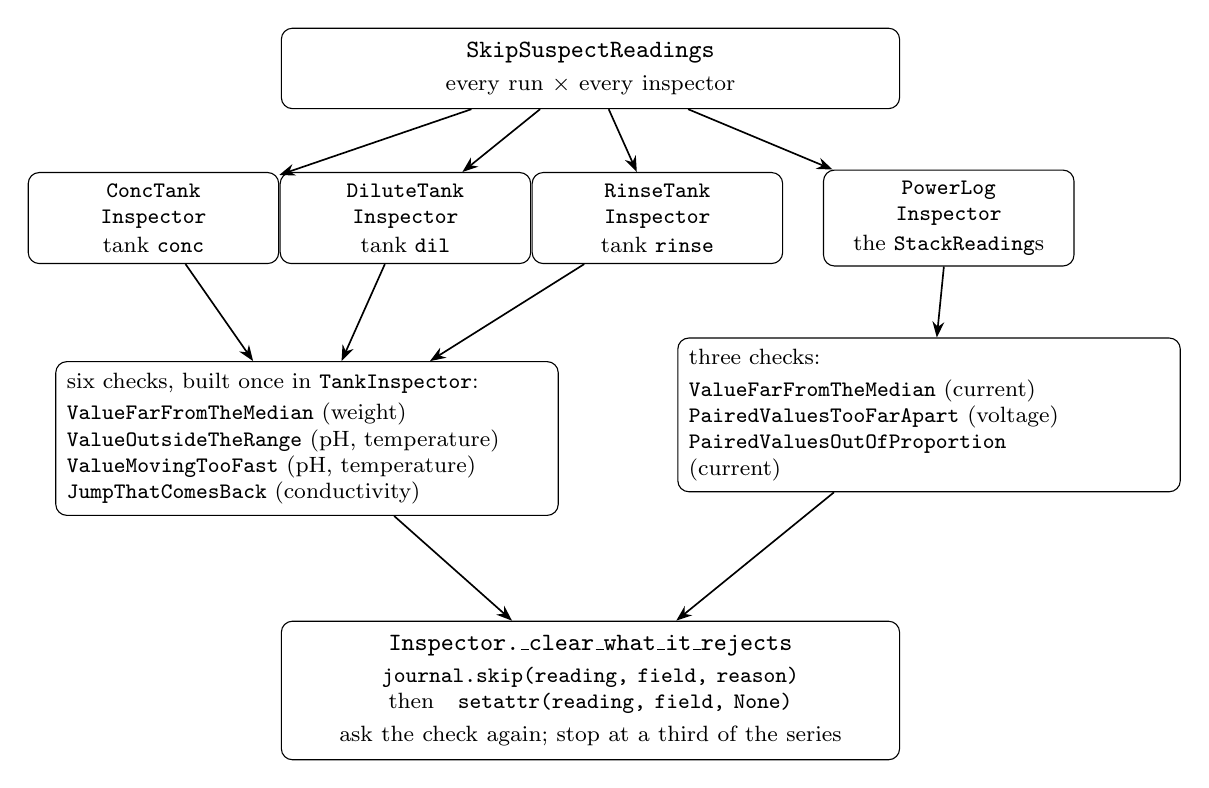
\begin{tikzpicture}[
  scale=1, transform shape,
  insp/.style={draw, rounded corners, align=center, font=\footnotesize, text width=2.9cm,
              inner sep=4pt},
  wide/.style={draw, rounded corners, align=center, font=\small, text width=7.5cm,
               inner sep=5pt},
  leaf/.style={draw, rounded corners, align=left, font=\footnotesize, text width=6.1cm,
               inner sep=4pt},
  flow/.style={-Stealth, semithick}
]

\node[wide] (step) at (0,0)
  {\texttt{SkipSuspectReadings}\\[1pt]
   \footnotesize every run $\times$ every inspector};

\node[insp] (conc) at (-5.55,-1.9) {\texttt{ConcTank}\\\texttt{Inspector}\\[1pt] tank
  \texttt{conc}};
\node[insp] (dil)  at (-2.35,-1.9) {\texttt{DiluteTank}\\\texttt{Inspector}\\[1pt] tank
  \texttt{dil}};
\node[insp] (rin)  at ( 0.85,-1.9) {\texttt{RinseTank}\\\texttt{Inspector}\\[1pt] tank
  \texttt{rinse}};
\node[insp] (pow)  at ( 4.55,-1.9) {\texttt{PowerLog}\\\texttt{Inspector}\\[1pt] the
  \texttt{StackReading}s};

\foreach \b in {conc, dil, rin, pow} \draw[flow] (step) -- (\b);

\node[leaf] (tankchecks) at (-3.6,-4.7)
  {six checks, built once in \texttt{TankInspector}:\\[2pt]
   \texttt{ValueFarFromTheMedian} (weight)\\
   \texttt{ValueOutsideTheRange} (pH, temperature)\\
   \texttt{ValueMovingTooFast} (pH, temperature)\\
   \texttt{JumpThatComesBack} (conductivity)};

\node[leaf] (powchecks) at (4.3,-4.4)
  {three checks:\\[2pt]
   \texttt{ValueFarFromTheMedian} (current)\\
   \texttt{PairedValuesTooFarApart} (voltage)\\
   \texttt{PairedValuesOutOfProportion}\\(current)};

\foreach \b in {conc, dil, rin} \draw[flow] (\b) -- (tankchecks);
\draw[flow] (pow) -- (powchecks);

\node[wide] (clear) at (0,-7.9)
  {\texttt{Inspector.\_clear\_what\_it\_rejects}\\[2pt]
   \footnotesize \texttt{journal.skip(reading, field, reason)}\quad then\quad
   \texttt{setattr(reading, field, None)}\\[1pt]
   \footnotesize ask the check again; stop at a third of the series};

\draw[flow] (tankchecks) -- (clear);
\draw[flow] (powchecks) -- (clear);

\end{tikzpicture}
\caption{Inside \texttt{SkipSuspectReadings}. The three tank inspectors differ only in which
tank they read; their checks are built once in the shared \texttt{TankInspector}. Every
threshold the checks compare against lives in \texttt{Thresholds}, and a value is cleared in
one place only.}
\label{fig:inspectors}
\end{figure}

\subsection{What each stage is responsible for}

\textbf{\texttt{DataLoader}} is the only part of the program that knows where the data lives.
It reads four tables, validates each against a pandera schema, groups the readings by run,
attaches each lab sample to the tank reading drawn at that minute, and hands back a list of
\texttt{Run} objects. It turns every blank cell into \texttt{None}, because pandas calls a
blank \texttt{NaN} and \texttt{NaN} would quietly survive arithmetic. Which source it uses
comes from \texttt{config.DATA\_SOURCE}, so moving the data out of CSV files is a
configuration change.

\textbf{\texttt{Preprocessor}} decides which runs the modelling may see and which individual
values it may trust. It saves nothing and prints nothing: it returns the surviving runs and
writes what it removed to the journal. It hands on \texttt{Run} objects of exactly the same
type it was given, which is what lets the steps chain.

\textbf{\texttt{Calculator}} is where the readings stop being readings. For each run it
works out the two settings, the two outcomes, and five diagnostics, and packs them into a
frozen \texttt{Result}. Nothing in a \texttt{Result} is copied from a CSV file; every field
was worked out. It drops a run only when one of the two fitted outcomes could not be had,
because a run with no permselectivity and no recovery has nothing to contribute. A missing
diagnostic is not a reason to drop: the command names those runs at the end instead.

\textbf{\texttt{Surrogate}} groups the results by membrane and, for each membrane with at
least three runs, fits all three outcomes and then searches. The fitting is delegated:
\texttt{DesignPoints} logs and codes the settings, \texttt{SecondOrderPolynomial} does the
least squares, \texttt{LeaveOneOutError} scores it, \texttt{ReplicateScatter} works out what
the bench's own repeats cost, and \texttt{FittedOutcome} holds all of it together. It writes
nothing to the journal: a membrane it will not fit is reported on its answer, with the
reason, because a membrane left out names the next experiment worth running.

On the current data this is where equation~\ref{eq:coded} is chosen. \texttt{FittedOutcome}
starts with an intercept alone and adds whichever single term lowers the leave-one-out error
most, stopping when nothing lowers it:

\begin{center}
\begin{tabular}{llrl}
\toprule
model so far & term offered & leave-one-out rmse & \\
\midrule
intercept                 & ---       & 15.0521 & the starting point \\
intercept                 & $x_1$     & 16.2443 & worse \\
intercept                 & $x_2$     & \textbf{7.8979} & best of the two, so $x_2$ is kept \\
intercept, $x_2$          & $x_1$     & 9.9497 & worse \\
intercept, $x_2$          & $x_2^2$   & \textbf{7.1218} & better, so $x_2^2$ is kept \\
intercept, $x_2$, $x_2^2$ & $x_1$     & 9.4710 & worse than 7.1218, so the model stops \\
\bottomrule
\end{tabular}
\end{center}

A squared term may only be offered once its own linear term is already in, since a curve
without its slope cannot be read. That is why $x_1^2$ never appears: $x_1$ never got in.

\textbf{\texttt{BestSetupUnderTheGates}} sweeps a $21 \times 21$ grid of coded points, keeps
those predicted to clear a recovery floor of $35\%$ and a voltage ceiling of
$20\unit{V}$, and returns the survivor with the highest predicted permselectivity. It sweeps
only inside the measured range, so the answer is always a setup the bench has evidence for.
On this data all 441 points fail the recovery floor and none fails the voltage ceiling: the
highest recovery the fit predicts anywhere in range is $33.28\%$. Nothing surviving is
reported as a finding with the blamed gate named, not as an error.

\textbf{\texttt{Analyze}} prints. The exclusions come first on purpose, so a reader who sees
the answer already knows how many runs it came from. Beside each equation it prints the
fit's leave-one-out error next to the bench scatter, and says outright when the error is
worse. For recovery it is: off by $7.122$ against a bench scatter of $6.612$ from two
repeats. The line the command adds is that this is worse than the bench repeating itself,
\emph{so this fit has earned no conclusion}.

\subsection{The one rule: a value that cannot be worked out becomes \texttt{None}}

One rule holds from the loader to the search, and it is the reason the code reads the way it
does. \textbf{A value that cannot be worked out becomes \texttt{None}, and is never guessed
at.} There is no imputation anywhere, no filling forward, no substituting a mean, no
treating a blank as zero.

It shows up at every level:

\begin{itemize}[nosep]
  \item the loader turns a blank cell into \texttt{None}, never $0$ --- a blank means
        \emph{not measured};
  \item a check clears a value it cannot believe, and \texttt{find\_judgeable\_readings}
        then passes over it, so a cleared value is absent rather than wrong;
  \item every quantity returns \texttt{None} rather than a partial answer:
        \texttt{VolumeInATank} with no weight, \texttt{FeedRatio} with no magnesium,
        \texttt{DesignPoints} on a setting at or below zero, which has no logarithm;
  \item \texttt{SecondOrderPolynomial.find\_fit} returns \texttt{None} when the design
        matrix comes back rank-deficient, because two terms moving together over these rows
        means no one set of coefficients is \emph{the} answer;
  \item \texttt{find\_prediction} returns \texttt{None} on an unfitted polynomial, and
        \texttt{BestSetupUnderTheGates} treats a point it cannot predict as a point it
        cannot judge rather than a point that passes.
\end{itemize}

The cost of the rule is that every caller has to check. The benefit is that no number in the
printed report was invented, and a gap in the bench record stays a gap all the way to the
page. The journal is the other half of the same rule: nothing is dropped or cleared without
a line saying what and why.

\subsection{The stages at a glance}

\begin{center}
\footnotesize
\begin{tabular}{@{}>{\raggedright\arraybackslash}p{2.1cm}>{\raggedright\arraybackslash}p{3.7cm}>{\raggedright\arraybackslash}p{3.2cm}>{\raggedright\arraybackslash}p{5.0cm}@{}}
\toprule
stage & the class that does it & takes in & hands on \\
\midrule
load &
  \texttt{DataLoader}, \texttt{CsvSource}, pandera schemas &
  four CSV files &
  21 \texttt{Run} objects, readings and samples attached \\
\addlinespace
preprocess &
  \texttt{Preprocessor} and its four \texttt{Step}s &
  21 \texttt{Run} objects &
  9 \texttt{Run} objects, 10 values cleared; drops and skips in the journal \\
\addlinespace
check a reading &
  \texttt{SkipSuspectReadings}, four \texttt{Inspector}s, six \texttt{Check} classes,
  \texttt{Thresholds} &
  one run's readings &
  the same readings, with unbelievable values set to \texttt{None} \\
\addlinespace
calculate &
  \texttt{Calculator} and the \texttt{quantities} package &
  9 \texttt{Run} objects &
  9 frozen \texttt{Result}s: two settings, two outcomes, five diagnostics \\
\addlinespace
code the settings &
  \texttt{DesignPoints} &
  the settings of each \texttt{Result} &
  one $(x_1, x_2)$ per run, logged, centred and scaled to $-1..1$, and the way back \\
\addlinespace
fit &
  \texttt{FittedOutcome}, \texttt{SecondOrderPolynomial}, \texttt{LeaveOneOutError},
  \texttt{ReplicateScatter} &
  coded rows and one outcome column &
  the terms that earned their place, their coefficients, the error, the bench scatter \\
\addlinespace
search &
  \texttt{BestSetupUnderTheGates} &
  three fitted outcomes and the design &
  the best setup in $\mathrm{mA/cm^2}$ and $\mathrm{mol/mol}$, or the gate that refused
  every point \\
\addlinespace
assemble &
  \texttt{Surrogate}, \texttt{SurrogateModels}, \texttt{Analysis} &
  9 \texttt{Result}s &
  fits and best setups per membrane, plus the membranes not fitted and why \\
\addlinespace
report &
  \texttt{Analyze} &
  the \texttt{Analysis} and the \texttt{Journal} &
  printed lines: exclusions, the run table, the fits, the thin runs \\
\bottomrule
\end{tabular}
\end{center}

\clearpage
\section{From a weight on a scale to a recovery percentage}

Two different equations in this project both call themselves the recovery model, and they
look nothing alike. Before anything else, here is which is which.

The equation this report is about is fitted in \emph{real units}, with current density $J$ in
$\mathrm{mA/cm^2}$ and the feed ratio $R$ in $\mathrm{mol/mol}$, and it keeps all five terms
that these runs can settle:

\begin{equation}
  \text{recovery \%} = 33.0192 + 3.16999\,J - 14.4538\,R - 0.0954576\,J^{2} + 0.837907\,R^{2}
  \label{eq:real-units-one-run}
\end{equation}

The equation \texttt{uv run limodel analyze} prints is not that one. The code logs both
settings, codes them onto $-1\ldots1$, and then chooses its terms by forward stepwise
selection, so it drops every term that does not lower the leave-one-out error. What it prints
is

\begin{equation}
  \text{recovery \%} = 11.5776 - 15.627\,x_{2} + 6.08016\,x_{2}^{2},
  \qquad x_{2} = \frac{\ln R - 1.395778}{1.039721}
  \label{eq:coded-units-fit}
\end{equation}

Different units, different terms, and no current density at all in \eqref{eq:coded-units-fit}.
The next section sets them side by side. What matters here is that
\eqref{eq:real-units-one-run} and \eqref{eq:coded-units-fit} are fitted to \emph{the same nine
numbers} on the left-hand side: nine measured recovery percentages, one per GO-10 run. Neither
equation can be better than those nine numbers, so this section takes one of them apart
completely. Run AE's recovery is $38.27\%$. Below is every reading that figure is made of and
every multiplication done to it, so it can be checked on paper.

\subsection{The rows AE's recovery is built from}

Nothing in the data files is a recovery percentage. Four raw rows across three CSV files hold
everything \eqref{eq:real-units-one-run} is fitted to for run AE, and Table~\ref{tab:ae-raw-rows}
is all of them. The tares come from the run sheet, the weights from the balance under each
tank, the concentrations from the lab.

\begin{table}[htbp]
\centering
\caption{The raw rows behind AE's recovery, as they sit in the data files. The two tares are
columns of AE's own row in \texttt{runs.csv}; each tank weight is a row of
\texttt{tank\_readings.csv}; each concentration is a row of \texttt{samples.csv}.}
\label{tab:ae-raw-rows}
\begin{tabular}{llrr}
\toprule
file & column or row & minute 0 & minute 240 \\
\midrule
\texttt{runs.csv}          & \texttt{tare\_conc\_g}  & \multicolumn{2}{c}{$96.2\unit{g}$} \\
                           & \texttt{tare\_dil\_g}   & \multicolumn{2}{c}{$111.5\unit{g}$} \\
\addlinespace
\texttt{tank\_readings.csv}& concentrate \texttt{weight\_g} & $2119.7\unit{g}$ & $2101.5\unit{g}$ \\
                           & dilute \texttt{weight\_g}      & $2117.8\unit{g}$ & $2040.7\unit{g}$ \\
\addlinespace
\texttt{samples.csv}       & concentrate \texttt{li\_mg\_l}
                           & $63.56\unit{mg/L}$ & $218.5\unit{mg/L}$ \\
                           & dilute \texttt{li\_mg\_l}
                           & $403.1\unit{mg/L}$ & $261.9\unit{mg/L}$ \\
\bottomrule
\end{tabular}
\end{table}

Two of the eight entries never reach recovery. The dilute's minute 240 weight and lithium are
in the table only to be set aside: recovery divides by what the feed held \emph{before}
anything moved, so only the dilute's first sampled minute is used. Its last minute is read by
the balance gap, which is a diagnostic and is never fitted.

\subsection{Weights become litres}

No instrument measured a volume. Each tank sat on a balance for the whole run, so the litres
are inferred: the balance reading less that tank's own empty weight, divided by
$1000\unit{g/L}$. \texttt{VolumeInATank.find\_litres} does this, and the divisor is
\texttt{SOLUTION\_\allowbreak G\_\allowbreak PER\_\allowbreak L} $= 1000.0$ in \texttt{calculate/\allowbreak constants.py}. That constant is a
decision, not a measurement. These are dilute salt solutions, so a litre weighs a kilogram
closely enough that the balance can be read as a volume, and the alternative --- a density per
tank per minute --- was never measured.

The concentrate is weighed at both ends, so it needs two volumes:

\begin{align}
  V_{\mathrm{conc}}(0)   &= \frac{2119.7 - 96.2}{1000} = 2.0235\unit{L} \label{eq:v-conc-0} \\
  V_{\mathrm{conc}}(240) &= \frac{2101.5 - 96.2}{1000} = 2.0053\unit{L} \label{eq:v-conc-240}
\end{align}

The tare is looked up by tank name through \texttt{TARE\_FIELD\_BY\_TANK}, which maps
\texttt{conc} to the column \texttt{tare\_conc\_g}; \texttt{AmountThatCrossed.find\_ends} is
what reads it off the run. The two volumes differ by $18.2\unit{g}$ of liquid, nine parts in a
thousand. That is small, and it is exactly why the volume is recomputed at each sampled minute
instead of once: a concentration at minute 240 compared against a minute 0 volume would be
comparing two different quantities of liquid.

\subsection{Litres and a lab result become milligrams}

A concentration on its own says nothing that can be compared across a run, because the tanks
gain and lose liquid all the way through. Only concentration times volume --- an absolute
amount --- can be subtracted from one minute to the next.
\texttt{AmountInATank.find\_milligrams} does the multiplication, taking the lithium column
name from \texttt{LITHIUM.field\_name}, which is \texttt{li\_mg\_l}:

\begin{align}
  m_{\mathrm{conc}}(0)   &= 63.56 \times 2.0235 = 128.61366\unit{mg} \label{eq:mg-conc-0} \\
  m_{\mathrm{conc}}(240) &= 218.5 \times 2.0053 = 438.15805\unit{mg} \label{eq:mg-conc-240}
\end{align}

The concentrate did not start empty of lithium. It was made up as $0.5\unit{g/L}$ LiCl, so
\eqref{eq:mg-conc-0} is not a rounding artefact and cannot be skipped --- about $29\%$ of what
the concentrate finished with was already in it. What crossed the membranes is the difference,
and \texttt{AmountThatCrossed.\allowbreak find\_milligrams} is the subtraction:

\begin{equation}
  \Delta m_{\mathrm{conc}} = 438.15805 - 128.61366 = 309.54439\unit{mg}
  \label{eq:crossed}
\end{equation}

The two ends are picked by minute and not by row order.
In \texttt{AmountThatCrossed}, the method
\texttt{find\_amounts\_by\_minute} builds a dictionary keyed on the minute, keeping only
the minutes that have both a weight and a lab result, and \texttt{find\_ends} then sorts
those keys and takes the first and the last. The readings arrive in no guaranteed order, and
most minutes of AE have a weight but no sample, so taking the first and last \emph{rows}
would pick up the wrong pair.

\subsection{The feed side, and the percentage}

The denominator is the whole prize: all the lithium the feed held when the run began. It is
built the same way, from the dilute tank's own tare and its first sampled minute:

\begin{align}
  V_{\mathrm{dil}}(0) &= \frac{2117.8 - 111.5}{1000} = 2.0063\unit{L} \label{eq:v-dil-0} \\
  m_{\mathrm{dil}}(0) &= 403.1 \times 2.0063 = 808.73953\unit{mg} \label{eq:mg-dil-0}
\end{align}

\texttt{LithiumRecovery.find\_percent} then divides \eqref{eq:crossed} by
\eqref{eq:mg-dil-0}:

\begin{equation}
  \text{recovery \%} = 100 \times \frac{309.54439}{808.73953} = 38.2749\%
  \label{eq:recovery}
\end{equation}

Three things about \eqref{eq:recovery} were choices. First, the denominator is the dilute's
\emph{first} sampled minute and never its last: measured against what the feed ended with,
AE would read $61.3\%$, which would be a share of what was left rather than a recovery.
Second, the numerator is what the \emph{concentrate gained}, not what the dilute lost --- the
concentrate is where the product is, and the dilute also loses lithium to the rinse and to the
sample bottles. Those two numbers disagree by a measurable amount, and the gap between them is
reported separately as a diagnostic rather than averaged away. Third, milligrams stand on both
sides of the division, so lithium's molar mass cancels and the code never converts to moles
here; recovery is the one quantity in the project that needs no molar mass at all.

Figure~\ref{fig:ae-recovery-chain} is the whole chain with these numbers on it.

\begin{figure}[htbp]
\centering
\footnotesize
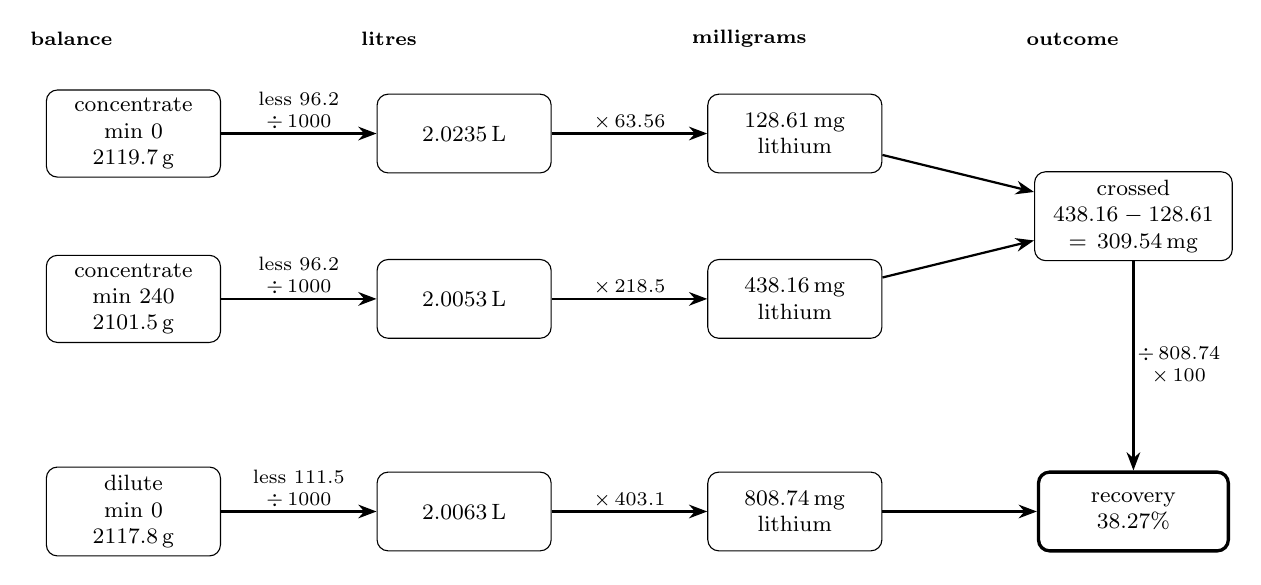
\begin{tikzpicture}[
  every node/.style={font=\footnotesize},
  box/.style={draw, rounded corners, align=center, text width=2.0cm, inner sep=3pt,
              minimum height=1.0cm},
  lbl/.style={font=\scriptsize, align=center, inner sep=1pt},
  arr/.style={-Stealth, thick}
]

\node[box] (cw0) at (0,2.5) {concentrate\\min 0\\$2119.7\unit{g}$};
\node[box] (cw4) at (0,0.4) {concentrate\\min 240\\$2101.5\unit{g}$};
\node[box] (dw0) at (0,-2.3) {dilute\\min 0\\$2117.8\unit{g}$};

\node[box] (cv0) at (4.2,2.5) {$2.0235\unit{L}$};
\node[box] (cv4) at (4.2,0.4) {$2.0053\unit{L}$};
\node[box] (dv0) at (4.2,-2.3) {$2.0063\unit{L}$};

\node[box] (cm0) at (8.4,2.5) {$128.61\unit{mg}$\\lithium};
\node[box] (cm4) at (8.4,0.4) {$438.16\unit{mg}$\\lithium};
\node[box] (dm0) at (8.4,-2.3) {$808.74\unit{mg}$\\lithium};

\node[box, text width=2.3cm] (cross) at (12.7,1.45)
  {crossed\\$438.16 - 128.61$\\$= 309.54\unit{mg}$};
\node[box, text width=2.2cm, very thick] (rec) at (12.7,-2.3) {recovery\\$38.27\%$};

\draw[arr] (cw0) -- node[lbl, above] {less $96.2$\\$\div\,1000$} (cv0);
\draw[arr] (cw4) -- node[lbl, above] {less $96.2$\\$\div\,1000$} (cv4);
\draw[arr] (dw0) -- node[lbl, above] {less $111.5$\\$\div\,1000$} (dv0);

\draw[arr] (cv0) -- node[lbl, above] {$\times\,63.56$} (cm0);
\draw[arr] (cv4) -- node[lbl, above] {$\times\,218.5$} (cm4);
\draw[arr] (dv0) -- node[lbl, above] {$\times\,403.1$} (dm0);

\draw[arr] (cm4) -- (cross);
\draw[arr] (cm0) -- (cross);
\draw[arr] (cross) -- node[lbl, right] {$\div\,808.74$\\$\times\,100$} (rec);
\draw[arr] (dm0) -- (rec);

\node[lbl, anchor=west] at (-1.35,3.7) {\textbf{balance}};
\node[lbl, anchor=west] at (2.85,3.7) {\textbf{litres}};
\node[lbl, anchor=west] at (7.05,3.7) {\textbf{milligrams}};
\node[lbl, anchor=west] at (11.3,3.7) {\textbf{outcome}};

\end{tikzpicture}
\caption{Run AE's recovery, every step with its own number. The tares come from
\texttt{runs.csv}, the weights from \texttt{tank\_readings.csv}, the multipliers from the
lithium column of \texttt{samples.csv}. Left to right the classes are
\texttt{VolumeInATank}, \texttt{AmountInATank}, \texttt{AmountThatCrossed} and
\texttt{LithiumRecovery}.}
\label{fig:ae-recovery-chain}
\end{figure}

\subsection{Permselectivity, which needs magnesium and the charge}

Recovery only asks how much lithium moved. Permselectivity asks whether the stack
\emph{preferred} lithium, which takes magnesium as well, and it has one wrinkle recovery does
not: it is about charge, not about ions.

The magnesium that crossed comes through exactly the same chain. The only change is the
column read, \texttt{MAGNESIUM.field\_name}, which is \texttt{mg\_mg\_l}:

\begin{equation}
  \Delta m_{\mathrm{Mg}} = 130.0 \times 2.0053 \;-\; 2.974 \times 2.0235
  = 260.689 - 6.01789 = 254.67111\unit{mg}
  \label{eq:crossed-mg}
\end{equation}

\texttt{TransportNumbers.find\_numbers} then converts both to millimoles and weights each by
the charge its own ion carries --- \texttt{Metal.charge}, which is $1$ for lithium and $2$ for
magnesium. Magnesium counts twice because a transport number is a share of the charge the
current carried, and one $\mathrm{Mg}^{2+}$ ion carries two charges across the membrane where
one $\mathrm{Li}^{+}$ carries one. The current is what was paid for, so the current is what
gets divided up:

\begin{align}
  q_{\mathrm{Li}} &= 1 \times \frac{309.54439}{6.94}   = 44.60294 \label{eq:q-li} \\
  q_{\mathrm{Mg}} &= 2 \times \frac{254.67111}{24.305} = 20.95627 \label{eq:q-mg} \\
  t_{\mathrm{Li}} &= \frac{44.60294}{65.55921} = 0.680346,
  \qquad t_{\mathrm{Mg}} = \frac{20.95627}{65.55921} = 0.319654 \label{eq:transport}
\end{align}

So lithium carried $68\%$ of the charge into the concentrate. On its own that number says
little, because AE's feed held more lithium than magnesium in molar terms and a stack with no
preference at all would still move mostly lithium. The feed it was offered has to be divided
out. \texttt{FeedRatio.find\_li\_over\_mg\_in\_the\_dilute} takes the first dilute minute the
lab reported both metals for, in millimoles. That minute is AE's minute 0, where the dilute
held $808.73953\unit{mg}$ of lithium by \eqref{eq:mg-dil-0} and
$1657 \times 2.0063 = 3324.4391\unit{mg}$ of magnesium:

\begin{equation}
  \frac{c_{\mathrm{Li}}}{c_{\mathrm{Mg}}}
  = \frac{808.73953 / 6.94}{3324.4391 / 24.305}
  = \frac{116.53307}{136.78005} = 0.851974
  \label{eq:feed-ratio}
\end{equation}

Both amounts are from one tank at one minute, so the litres cancel and the milligrams carry
the ratio --- which is why \eqref{eq:feed-ratio} divides milligrams-over-molar-mass directly.
\texttt{Permselectivity.\allowbreak find\_value} finishes it:

\begin{equation}
  P = \frac{t_{\mathrm{Li}} / t_{\mathrm{Mg}}}{c_{\mathrm{Li}} / c_{\mathrm{Mg}}}
    = \frac{0.680346 / 0.319654}{0.851974}
    = \frac{2.128381}{0.851974} = 2.498176
  \label{eq:permselectivity}
\end{equation}

\subsubsection*{Why no preference is $0.5$ and not $1$}

Dividing by the feed ratio is what lets runs fed different mixtures be compared, and it fixes
the neutral point at $0.5$ whatever the feed was. The reason is the factor of two in
\eqref{eq:q-mg}, which survives the division.

Suppose the stack had no preference, so the ions crossed in proportion to the moles offered:
$n_{\mathrm{Li}} / n_{\mathrm{Mg}} = c_{\mathrm{Li}} / c_{\mathrm{Mg}}$. The transport numbers
are charge shares, so

\begin{equation}
  \frac{t_{\mathrm{Li}}}{t_{\mathrm{Mg}}}
  = \frac{1 \cdot n_{\mathrm{Li}}}{2 \cdot n_{\mathrm{Mg}}}
  = \frac{1}{2}\,\frac{c_{\mathrm{Li}}}{c_{\mathrm{Mg}}},
  \qquad\text{so}\qquad
  P = \frac{\tfrac{1}{2}\,(c_{\mathrm{Li}} / c_{\mathrm{Mg}})}{c_{\mathrm{Li}} / c_{\mathrm{Mg}}}
    = \frac{1}{2}
  \label{eq:neutral-point}
\end{equation}

The feed ratio cancels completely, so $0.5$ is the neutral point for every run regardless of
what it was fed. For AE, no preference would have meant
$t_{\mathrm{Li}} / t_{\mathrm{Mg}} = 0.851974 / 2 = 0.425987$; the stack actually reached
$2.128381$, about five times that, hence $P = 2.498$ against a neutral $0.5$. Read against $1$
instead, the same stack would look only $2.5$ times selective rather than $5$, so the neutral
point has to be stated with the number.

One more thing about \eqref{eq:feed-ratio}: it is the \emph{measured} feed ratio, from the lab
result on the dilute sample. It is not the ratio the run was set up at. AE was made up at
$400\unit{mg/L}$ lithium and $2000\unit{mg/L}$ magnesium, which is
$(2000/24.305) / (400/6.94) = 1.427690$ mol magnesium per mole lithium, or $0.700432$ the
other way up --- not $0.851974$. \texttt{FeedRatio} keeps the two apart by name,
\texttt{find\_li\_over\_mg\_in\_the\_dilute} against
\texttt{find\_mg\_over\_li\_from\_the\_setup}, because they answer different questions. The
measured one is what permselectivity divides by, since it is the mixture the membrane actually
saw. The set-up one is the design column $R$ of \eqref{eq:real-units-one-run}, since a design
column has to be a setting the bench chose and can choose again, not something a lab result
moves afterwards.

\subsection{What else a \texttt{Result} carries}

\texttt{Calculator.find\_results} builds one \texttt{Result} per run, and it drops a run only
when permselectivity or recovery could not be worked out --- those two are what the model is
fitted to, so a run without them has nothing to contribute. The rest may be \texttt{None} on a
run that is otherwise sound, which is why they are reported at the end rather than used to
drop anything. Table~\ref{tab:result-fields} names each field, the class behind it, and what
AE came out as.

\begin{table}[htbp]
\centering
\caption{Every field of a \texttt{Result} beyond the two derived above, with the class that
produces it and AE's value. The last five are diagnostics: read by a human judging a run,
never fitted.}
\label{tab:result-fields}
\begin{tabular}{llr}
\toprule
field & class and method & AE \\
\midrule
\texttt{current\_density\_ma\_cm2} & \texttt{CurrentDensity.find\_ma\_per\_cm2} & $13.6667$ \\
\texttt{feed\_mg\_li\_ratio}
  & \texttt{FeedRatio.find\_mg\_over\_li\_from\_the\_setup} & $1.42769$ \\
\addlinespace
\texttt{highest\_voltage\_v} & \texttt{StackVoltage.find\_highest\_volts} & $16.0\unit{V}$ \\
\texttt{charge\_passed\_mah\_cm2} & \texttt{ChargeThatPassed.find\_mah\_per\_cm2} & $54.5625$ \\
\texttt{energy\_per\_mol\_li\_wh} & \texttt{EnergyPerMoleOfLithium.find\_watt\_hours} & $91.92$ \\
\texttt{li\_balance\_gap\_pct} & \texttt{BalanceGap.find\_percent} & $-19.64\%$ \\
\texttt{mg\_balance\_gap\_pct} & \texttt{BalanceGap.find\_percent} & $35.00\%$ \\
\bottomrule
\end{tabular}
\end{table}

Four of these are worth a line on why they are shaped the way they are.

\textbf{Current density} is the \emph{median} supply current over the power log, times $1000$
for milliamps, divided by the membrane area. AE's power log carries a current at 30
minutes, 25 of them $0.082\unit{A}$, so $0.082 \times 1000 / 6 = 13.6667\unit{mA/cm^2}$.
The median and not the
mean, because a run holds one current all the way through and a single misread minute should
not shift the number that labels the whole run. This is the $J$ of
\eqref{eq:real-units-one-run}.

\textbf{Highest voltage} is the largest voltage the log ever recorded, which is what the
$20\unit{V}$ ceiling is checked against. \texttt{StackVoltage} also offers
\texttt{find\_starting\_volts}, the voltage at the earliest logged minute, which is what the
stack asked for before anything had crossed.

\textbf{Charge passed} and \textbf{energy per mole} are both areas under the power log, found
by the trapezium rule between consecutive logged minutes, because no meter totalled either
one. AE integrates to $1178.55\unit{C}$, which over $6\unit{cm^2}$ is
$54.5625\unit{mAh/cm^2}$, and to $14759.78\unit{J}$, which against the
$309.54\unit{mg} / 6.94 = 44.6\unit{mmol}$ of lithium that crossed is
$91.92\unit{Wh}$ per mole. Per mole of lithium rather than per hour or per litre, so a short
run and a long one can be set beside each other.

\textbf{The balance gaps} are the honest confession of the chain above. Each one is the
percent of what the dilute lost that was not found again in the concentrate plus the rinse.
AE's lithium gap is $-19.64\%$: more lithium was found than the dilute appears to have lost,
which is a measurement inconsistency and not a physical one. It is reported and never
corrected for, and no quantity in this project is adjusted by it. When the rinse was never
weighed it counts as zero gained, which can only make the gap look worse --- the honest
direction for a diagnostic to be wrong in.

With all of that, AE reduces to one row the fitting can see: $J = 13.6667$, $R = 1.42769$,
recovery $= 38.27\%$, permselectivity $= 2.498$. Nine such rows are everything
\eqref{eq:real-units-one-run} and \eqref{eq:coded-units-fit} were fitted to.

\clearpage
\section{Where the five numbers come from}

\subsection{Two equations, and which is which}

There are two polynomials in play, and they are not the same polynomial. Mixing them up
is the easiest mistake to make here, so they are set side by side before anything else.

The first is the one this section is about. It is an ordinary least squares fit to the nine
GO-10 runs, with the two settings left in the units the bench works in --- current density
$J$ in $\unit{mA/cm^2}$ and feed ratio $R$ in $\unit{mol/mol}$ --- and with all five
estimable terms fitted at once:
%
\begin{equation}
  \widehat{\text{recovery}}\,[\%] \;=\; 33.0192 \;+\; 3.16999\,J \;-\; 14.4538\,R
  \;-\; 0.0954576\,J^{2} \;+\; 0.837907\,R^{2}
  \label{eq:real-units-fit}
\end{equation}

The second is the one \texttt{uv run limodel analyze} prints. The code does not fit in real
units and does not fit every term. It takes the logarithm of each setting, centres and scales
it to run from $-1$ to $+1$ across the runs, and then grows the model one term at a time,
keeping a term only while it lowers the leave-one-out error. For recovery it stops with three
terms and prints
%
\begin{equation}
  \widehat{\text{recovery}}\,[\%] \;=\; 11.5776 \;-\; 15.627\,x_2 \;+\; 6.08016\,x_2^{2},
  \qquad x_2 = \frac{\ln R - 1.395778}{1.039721}
  \label{eq:coded-fit}
\end{equation}

Equation~\eqref{eq:coded-fit} has no $J$ in it at all. Equation~\eqref{eq:real-units-fit} is
not what the code reports; it is the plain, all-terms, real-units fit, written out so that
every coefficient in it can be traced to arithmetic on nine rows of measurements. That is
what the rest of this section does. Why the code works in logged, coded units and selects its
terms is a separate matter and is not argued here.

\subsection{The question least squares asks}

Nine runs survived preprocessing, all on the GO-10 membrane. Each one is three numbers: the
current density it was held at, the feed ratio it was fed, and the lithium recovery that came
out of it.

\begin{table}[htbp]
  \centering
  \caption{The nine GO-10 runs the fit is made from.}
  \label{tab:nine-runs}
  \begin{tabular}{llrr}
    \toprule
    Run & $J$ ($\mathrm{mA/cm^2}$) & $R$ ($\mathrm{mol/mol}$) & Recovery (\%) \\
    \midrule
    AE & 13.6667 & 1.4277  & 38.27 \\
    AF & 13.6667 & 2.8554  & 18.34 \\
    AG & 13.6667 & 5.7108  & 6.16  \\
    AH & 7.5000  & 1.4277  & 36.59 \\
    AI & 7.5000  & 1.4277  & 37.66 \\
    AJ & 4.5000  & 1.4277  & 21.08 \\
    AN & 25.6667 & 1.4277  & 39.50 \\
    AP & 25.6667 & 1.4277  & 26.32 \\
    AT & 13.6667 & 11.4215 & 2.32  \\
    \bottomrule
  \end{tabular}
\end{table}

We choose a shape for the answer first: a second order polynomial in the two settings. Then
we ask for the five numbers $b_0,\dots,b_4$ that make the nine predicted recoveries as close
as they can be to the nine measured ones. ``As close as they can be'' has to be made precise,
because there is no single set of five numbers that hits all nine measurements. Least squares
makes it precise in one particular way: add up the squares of the nine misses, and pick the
five numbers that make that total as small as possible.
%
\begin{equation}
  b \;=\; \arg\min_{b_0,\dots,b_4} \;\sum_{i=1}^{9}
  \Bigl( y_i - \bigl[\, b_0 + b_1 J_i + b_2 R_i + b_3 J_i^{2} + b_4 R_i^{2} \,\bigr] \Bigr)^{2}
  \label{eq:least-squares-question}
\end{equation}

Here $y_i$ is the recovery measured on run $i$. Squaring, rather than taking the size of the
miss, is a choice, and it is worth knowing it was made: squaring makes a miss of $6$ count
four times a miss of $3$, so the answer is pulled hard towards the runs it would otherwise
fit worst. It also makes the problem solvable in closed form, which is the next subsection.

\subsection{The design matrix}

Equation~\eqref{eq:least-squares-question} is tidier in matrix form. Put the nine measured
recoveries in a column $y$, and build a matrix $X$ with one row per run and one column per
term. Each column is a rule applied to that run's own $J$ and $R$:

\begin{itemize}[nosep]
  \item column 1 is the constant $1$, the same for every run --- this is what $b_0$ multiplies;
  \item column 2 is $J$, the run's current density, as recorded;
  \item column 3 is $R$, the run's feed ratio, as recorded;
  \item column 4 is $J^2$, that same current density times itself;
  \item column 5 is $R^2$, that same feed ratio times itself.
\end{itemize}

Nothing is standardised, logged or re-centred. The numbers in $X$ are the bench's numbers and
their squares, which is exactly why the coefficients in \eqref{eq:real-units-fit} carry real
units.

{\footnotesize
\setlength{\arraycolsep}{4pt}
\begin{equation}
  X \;=\;
  \begin{array}{r}
    \text{AE}\\ \text{AF}\\ \text{AG}\\ \text{AH}\\ \text{AI}\\
    \text{AJ}\\ \text{AN}\\ \text{AP}\\ \text{AT}
  \end{array}\!\!
  \begin{bmatrix}
    1 & 13.6667 & 1.4277  & 186.7778 & 2.0383   \\
    1 & 13.6667 & 2.8554  & 186.7778 & 8.1532   \\
    1 & 13.6667 & 5.7108  & 186.7778 & 32.6128  \\
    1 & 7.5000  & 1.4277  & 56.2500  & 2.0383   \\
    1 & 7.5000  & 1.4277  & 56.2500  & 2.0383   \\
    1 & 4.5000  & 1.4277  & 20.2500  & 2.0383   \\
    1 & 25.6667 & 1.4277  & 658.7778 & 2.0383   \\
    1 & 25.6667 & 1.4277  & 658.7778 & 2.0383   \\
    1 & 13.6667 & 11.4215 & 186.7778 & 130.4511
  \end{bmatrix},
  \qquad
  y \;=\;
  \begin{bmatrix}
    38.27 \\ 18.34 \\ 6.16 \\ 36.59 \\ 37.66 \\ 21.08 \\ 39.50 \\ 26.32 \\ 2.32
  \end{bmatrix}
  \label{eq:design-matrix}
\end{equation}
}

Two features of this matrix decide everything that follows. Rows AH and AI are identical, and
so are rows AN and AP: those are repeats, two runs at the same setting. Identical rows must
get identical predictions, whatever the five numbers turn out to be. And the right-hand column
is nearly all the same value: six of the nine runs sat at $R = 1.4277$, so the feed ratio was
only ever moved at one current density.

\subsection{Why five columns and not six}

A full second order model in two settings has six terms, the sixth being the interaction
$J\cdot R$. It is left out of $X$ because over these nine runs it cannot be fitted at all --
not because it was judged unimportant.

The runs move current density only at the lowest feed ratio, and move feed ratio only at one
current density. That cross shape makes the product column an exact combination of three
columns already present:
%
\begin{equation}
  J_i R_i \;=\; 1.42769\,J_i \;+\; 13.66667\,R_i \;-\; 19.51176
  \qquad \text{for all nine runs}
  \label{eq:interaction-identity}
\end{equation}

This is not approximately true, it is true: the largest discrepancy across the nine rows is
$7.1\times10^{-15}$, which is floating point noise and nothing else. Add $J\cdot R$ as a sixth
column and the matrix has rank 5, not 6. Six unknowns, five independent pieces of information:
infinitely many different sets of six coefficients would fit the nine runs equally well, so
there is no answer to report. The code meets the same wall and handles it by refusing the
fit --- \texttt{SecondOrderPolynomial.find\_fit} checks the rank \texttt{numpy} hands back and
returns \texttt{None} when it falls short of the number of terms.

\subsection{The normal equations}

Minimising a sum of squares is a calculus problem. Write the total squared miss as
$S(b) = (y - Xb)^{\mathsf T}(y - Xb)$ and differentiate it with respect to each of the five
coefficients in turn. At the minimum every one of those five derivatives is zero, which gives
five equations in the five unknowns:
%
\begin{equation}
  \frac{\partial S}{\partial b} \;=\; -2X^{\mathsf T}(y - Xb) \;=\; 0
  \qquad\Longrightarrow\qquad
  \bigl(X^{\mathsf T}X\bigr)\,b \;=\; X^{\mathsf T}y
  \label{eq:normal-equations}
\end{equation}

These are the normal equations. The name comes from what they say: the vector of misses
$y - Xb$ is at right angles --- normal --- to every column of $X$. That has a plain reading.
If the leftover misses still leaned one way with $J$, you could lower the total by adjusting
$b_1$, so you were not at the minimum. At the minimum there is no leaning left to exploit.

Both sides are small, and both are made of nothing but sums of products of the numbers in
\eqref{eq:design-matrix}. The top left entry of $X^{\mathsf T}X$ is $9$, the number of runs,
because it is the first column dotted with itself. The second entry of the top row is
$125.5$, which is the nine current densities added up.

{\footnotesize
\setlength{\arraycolsep}{4pt}
\begin{equation}
  X^{\mathsf T}X =
  \begin{bmatrix}
    9        & 125.5      & 28.5538   & 2197.4167    & 183.4468   \\
    125.5    & 2197.4167  & 393.8044  & 44962.6528   & 2512.2024  \\
    28.5538  & 393.8044   & 183.4468  & 6070.4973    & 1716.9338  \\
    2197.4167& 44962.6528 & 6070.4973 & 1014258.2616 & 35316.4021 \\
    183.4468 & 2512.2024  & 1716.9338 & 35316.4021   & 18172.4790
  \end{bmatrix},
  \qquad
  X^{\mathsf T}y =
  \begin{bmatrix}
    226.2459 \\ 3230.6772 \\ 398.8249 \\ 60119.2880 \\ 1060.2725
  \end{bmatrix}
  \label{eq:normal-matrices}
\end{equation}
}

Note how wide the range of magnitudes is: $9$ in one corner and $1{,}014{,}258$ in another.
That is what squaring a current density of $25.67$ twice over does, and it matters in the next
subsection.

\subsection{Solving them}

Solving \eqref{eq:normal-equations} with those numbers gives the five coefficients:
%
\begin{equation}
  b \;=\;
  \begin{bmatrix} b_0 \\ b_1 \\ b_2 \\ b_3 \\ b_4 \end{bmatrix}
  \;=\;
  \begin{bmatrix}
    33.019212 \\ 3.169987 \\ -14.453829 \\ -0.0954576 \\ 0.837907
  \end{bmatrix}
  \label{eq:coefficients}
\end{equation}

which is equation~\eqref{eq:real-units-fit}, written out. That is the whole answer to ``how
those numbers'': they are what you get when you form the two arrays in
\eqref{eq:normal-matrices} out of nine rows of bench data and solve a five by five linear
system.

A solver does not take that route. \texttt{SecondOrderPolynomial.\allowbreak find\_fit}
calls \texttt{numpy.\allowbreak linalg.\allowbreak lstsq}, which asks the same question ---
it is still \eqref{eq:least-squares-question} --- but answers it by singular value
decomposition of $X$ itself, without ever forming $X^{\mathsf T}X$. Hand the five real-unit
columns of \eqref{eq:design-matrix} to either route and they agree to
$1.07\times10^{-12}$, so for reading the coefficients it makes no difference which is used.
(The code is never handed those columns: \texttt{find\_fit} only ever sees the logged, coded
columns of \eqref{eq:coded-fit}. What is shared is the solver, not the fit.)

A solver prefers the decomposition route because forming $X^{\mathsf T}X$ squares the
condition number, the measure of how much a solution can move when the inputs are nudged.
For this $X$ the condition number is $1770$; for $X^{\mathsf T}X$ it is
$3.13\times10^{6}$. Multiplying the matrix by its own transpose throws away about half the
available precision before the solving even starts, for no gain.

\begin{figure}[htbp]
  \centering
  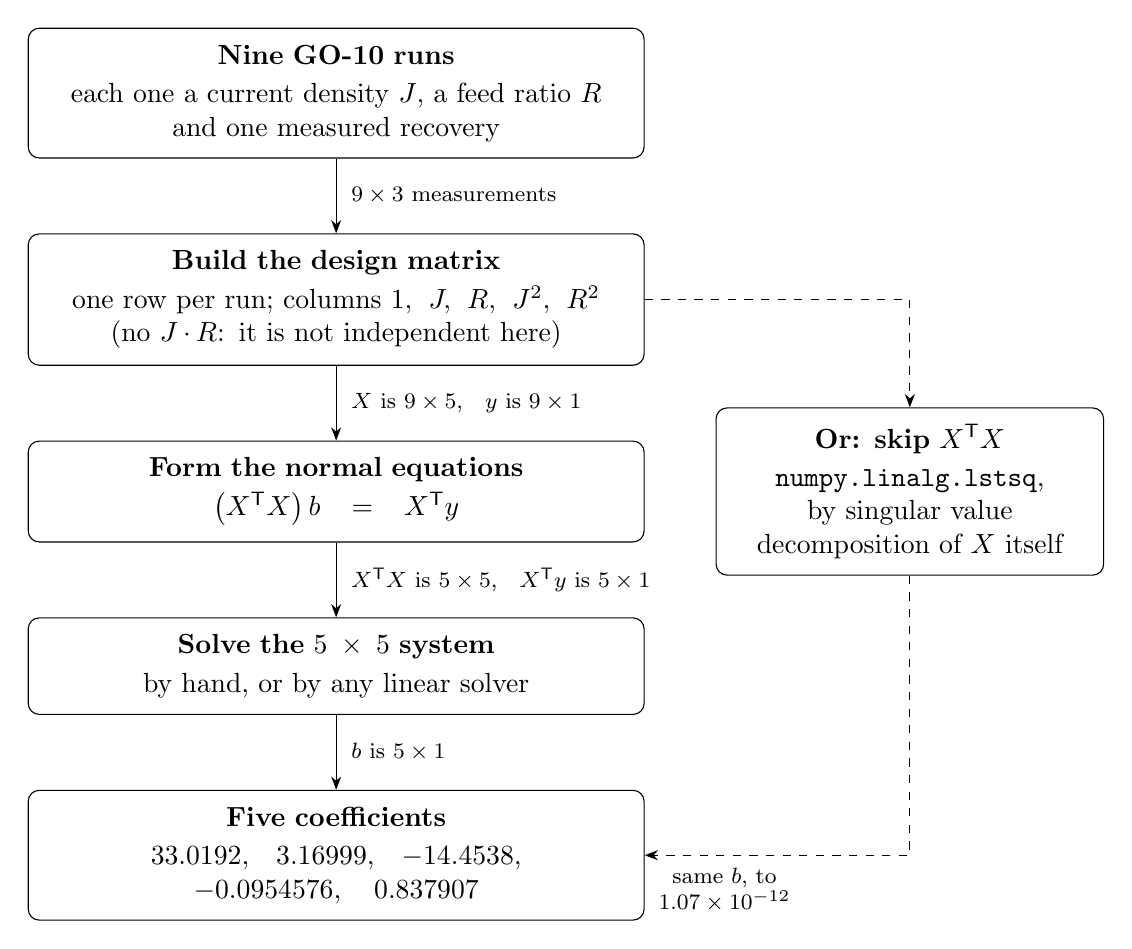
\begin{tikzpicture}[
      box/.style={draw, rounded corners, align=center, inner sep=6pt, text width=7.4cm},
      lab/.style={font=\footnotesize, align=left, xshift=2pt}
    ]
    \node[box] (runs)
      {\textbf{Nine GO-10 runs}\\[2pt]
       each one a current density $J$, a feed ratio $R$\\ and one measured recovery};
    \node[box, below=0.95cm of runs] (design)
      {\textbf{Build the design matrix}\\[2pt]
       one row per run; columns $1,\;J,\;R,\;J^{2},\;R^{2}$\\
       (no $J\!\cdot\!R$: it is not independent here)};
    \node[box, below=0.95cm of design] (normal)
      {\textbf{Form the normal equations}\\[2pt]
       $\bigl(X^{\mathsf T}X\bigr)\,b = X^{\mathsf T}y$};
    \node[box, below=0.95cm of normal] (solve)
      {\textbf{Solve the $5\times5$ system}\\[2pt]
       by hand, or by any linear solver};
    \node[box, right=0.9cm of normal, text width=4.5cm] (svd)
      {\textbf{Or: skip $X^{\mathsf T}X$}\\[2pt]
       \texttt{numpy.linalg.lstsq},\\ by singular value\\ decomposition of $X$ itself};
    \node[box, below=0.95cm of solve] (out)
      {\textbf{Five coefficients}\\[2pt]
       $33.0192,\;3.16999,\;-14.4538,$\\ $-0.0954576,\;0.837907$};

    \draw[-Stealth] (runs)   -- node[right, lab] {$9 \times 3$ measurements} (design);
    \draw[-Stealth] (design) --
      node[right, lab] {$X$ is $9 \times 5$, \; $y$ is $9 \times 1$} (normal);
    \draw[-Stealth] (normal) --
      node[right, lab] {$X^{\mathsf T}X$ is $5 \times 5$, \; $X^{\mathsf T}y$ is $5 \times 1$}
      (solve);
    \draw[-Stealth] (solve) -- node[right, lab] {$b$ is $5 \times 1$} (out);
    \draw[-Stealth, dashed] (design.east) -| (svd.north);
    \draw[-Stealth, dashed] (svd.south) |-
      node[pos=0.86, below, lab, align=center, yshift=-1pt]
        {same $b$, to\\ $1.07\times10^{-12}$} (out.east);
  \end{tikzpicture}
  \caption{From nine runs to five coefficients. The solid path is the one this section
    works through: the shapes on its arrows are where the nine runs stop being nine things,
    since once $X^{\mathsf T}X$ and $X^{\mathsf T}y$ are formed the problem is five by five
    no matter how many runs went in. The dashed path is what a solver actually does --- the
    same least squares question, decomposing $X$ directly and never forming
    $X^{\mathsf T}X$. Both land on the same five numbers. Neither is the equation
    \texttt{uv run limodel analyze} prints: that one is fitted on the coded columns of
    \eqref{eq:coded-fit}.}
  \label{fig:least-squares-flow}
\end{figure}

\subsection{What the answer means run by run}

Put each run's $J$ and $R$ back into \eqref{eq:real-units-fit} and you get what the equation
thinks that run should have given. The difference is the residual.

\begin{table}[htbp]
  \centering
  \caption{Measured, fitted and residual recovery for all nine runs, with each run's
    leverage --- how much of its own fitted value the run itself dictates.}
  \label{tab:fitted-and-residuals}
  \begin{tabular}{lrrrr}
    \toprule
    Run & Measured (\%) & Fitted (\%) & Residual (\%) & Leverage \\
    \midrule
    AE & 38.27 & 39.59 & $-1.31$ & 0.644 \\
    AF & 18.34 & 24.07 & $-5.73$ & 0.337 \\
    AG & 6.16  & 3.30  & $+2.86$ & 0.834 \\
    AH & 36.59 & 32.50 & $+4.09$ & 0.258 \\
    AI & 37.66 & 32.50 & $+5.16$ & 0.258 \\
    AJ & 21.08 & 26.42 & $-5.34$ & 0.677 \\
    AN & 39.50 & 32.57 & $+6.93$ & 0.499 \\
    AP & 26.32 & 32.57 & $-6.25$ & 0.499 \\
    AT & 2.32  & 2.73  & $-0.41$ & 0.997 \\
    \midrule
    \multicolumn{3}{l}{Sum of squared residuals} & \multicolumn{2}{r}{$201.9127$} \\
    \bottomrule
  \end{tabular}
\end{table}

$201.9127$ is the smallest that total can be made with five numbers of this shape. Any other
five numbers give a larger total; that is what \eqref{eq:least-squares-question} asked for and
what \eqref{eq:coefficients} delivers.

The residuals are not scattered at random, and the leverage column says why. Leverage is the
share of its own fitted value that a run dictates; the nine leverages add to $5$, one for each
coefficient, so they are literally how the five coefficients are spent across the nine runs.

Run AT, the single run at $R = 11.4215$, has leverage $0.997$. It is almost the only evidence
the $R^2$ column has at the far end of the feed ratio range, so the surface bends through it,
and its residual is $-0.41$. AG, the only run at $R = 5.7108$, is the next most influential at
$0.834$ and is fitted to $+2.86$. In other words, where the design has one run and no second
opinion, the fit passes close to it almost by obligation, not because the physics was captured.

The big residuals sit at the opposite end. Rows AH and AI of $X$ are the same row, so both get
the same prediction, $32.50$; rows AN and AP are the same row, so both get $32.57$. But the
bench measured $36.59$ and $37.66$ at the first setting and $39.50$ and $26.32$ at the second.
The fit splits each pair down the middle and the disagreement between the repeats lands
entirely in the residuals: $+4.09$, $+5.16$, $+6.93$, $-6.25$. No choice of five coefficients
can remove those, because the four misses are the bench disagreeing with itself.

One run does not follow the simple reading. AF is the only run at $R = 2.8554$ yet it has the
\emph{lowest} leverage of the nine, $0.337$, and the second largest residual, $-5.73$. Being
alone at a setting is not what buys influence; sitting at the edge of the range is. AF sits in
the middle of the feed ratio range, where the quadratic in $R$ is already pinned down by the
runs on either side of it, so the fit is free to miss it.

Whether a total of $201.9127$ is small enough to believe is the next section's question.

\subsection{Why the coefficients cannot be read one at a time}

It is tempting to read $b_1 = +3.17$ as ``more current gives more recovery'' and
$b_4 = +0.838$ as ``more magnesium in the feed gives more recovery''. Both readings are wrong,
and they are wrong for the same reason: in a polynomial, a coefficient has no meaning on its
own. $J$ and $J^2$ move together, always, so $b_1$ and $b_3$ only say something as a pair.

Differentiate \eqref{eq:real-units-fit} with respect to $J$ and the pair speaks:
%
\begin{equation}
  \frac{\partial\,\widehat{\text{recovery}}}{\partial J}
  \;=\; 3.16999 \;-\; 2 \times 0.0954576\,J
  \;=\; 0 \quad\text{at}\quad J = 16.60\unit{mA/cm^2}
  \label{eq:j-turning-point}
\end{equation}

A positive $b_1$ with a negative $b_3$ is a hump, not a slope. The fitted surface rises with
current density up to about $16.6\unit{mA/cm^2}$ and falls after it, and that turning point
sits inside the range the runs covered, $4.5$ to $25.67$. The same pair of numbers read
separately would have said the opposite things about the two halves of that curve.

The feed ratio pair behaves the other way round. $b_2 = -14.45$ with $b_4 = +0.838$ turns at
$R = 8.62\unit{mol/mol}$, so over most of the tested range the surface falls steeply with
feed ratio and then flattens out as it approaches the highest run. The positive $b_4$ is not a
benefit of magnesium; it is the flattening of a steep fall.

The honest way to quote a fit like this is never a coefficient. It is a predicted recovery at
a stated setting.

\begin{table}[htbp]
  \centering
  \caption{What equation~\eqref{eq:real-units-fit} predicts at real settings. Reading down
    the first block, current density has a best value rather than a direction; reading down
    the second, feed ratio dominates everything.}
  \label{tab:predictions-at-real-settings}
  \begin{tabular}{rrr}
    \toprule
    $J$ ($\mathrm{mA/cm^2}$) & $R$ ($\mathrm{mol/mol}$) & Predicted recovery (\%) \\
    \midrule
    4.5000  & 1.4277 & 26.42 \\
    7.5000  & 1.4277 & 32.50 \\
    13.6667 & 1.4277 & 39.59 \\
    16.6042 & 1.4277 & 40.41 \\
    25.6667 & 1.4277 & 32.57 \\
    \midrule
    13.6667 & 2.8554  & 24.07 \\
    13.6667 & 5.7108  & 3.30  \\
    13.6667 & 11.4215 & 2.73  \\
    \bottomrule
  \end{tabular}
\end{table}

Table~\ref{tab:predictions-at-real-settings} says something no single coefficient could. Over
the whole tested span of current density the prediction moves by about
14 percentage points, and it moves up and then back down. Over the tested span of feed ratio,
at fixed current density, it moves by about 37 percentage points, all downward. The
five numbers in \eqref{eq:coefficients} encode that, but only together.

\clearpage
\section{Whether that equation can be believed, and what the code fits instead}

Two different equations are in play, and they must not be confused with each other.

The first is the one asked about. It is ordinary least squares on the nine GO-10 runs, with
$J$ and $R$ in their real units, fitting all five estimable terms at once:

\begin{equation}
  \label{eq:five-term}
  \widehat{\text{recovery}}\;\%
  = 33.0192 + 3.16999\,J - 14.4538\,R - 0.0954576\,J^{2} + 0.837907\,R^{2}.
\end{equation}

The second is the one the code prints. It is a different fit: logged and coded units, and only
the terms that earned their place by forward stepwise selection.

\begin{equation}
  \label{eq:code-fit}
  \widehat{\text{recovery}}\;\%
  = 11.5776 - 15.627\,x_2 + 6.08016\,x_2^{2},
  \qquad x_2 = \frac{\ln R - 1.395778}{1.039721}.
\end{equation}

Equation~\eqref{eq:five-term} is a hand fit, made to answer the question ``what do five terms in
real units come to''. Equation~\eqref{eq:code-fit} is what \texttt{uv run limodel analyze} prints
today. They share the nine runs and nothing else: different units, different terms, different
column space. Current density does not appear in~\eqref{eq:code-fit} at all. The rest of this
section judges the first and then explains the second.

\subsection{$R^{2}$ says 0.875, and $R^{2}$ cannot say otherwise}

$R^{2}$ compares the squared misses of the fit against the squared misses of the flat line at
the mean. For~\eqref{eq:five-term} the sum of squared residuals is $201.9127$ and the same sum
about the mean of the nine recoveries is $1611.1333$, so

\begin{equation}
  R^{2} = 1 - \frac{201.9127}{1611.1333} = 0.875.
\end{equation}

That number is not evidence, because of how least squares works. Adding a column to $X$ widens
the space the fit may land in, and it still contains everything the narrower space contained ---
setting the new coefficient to zero recovers the old fit exactly. Least squares takes the best
point in the wider space, so the sum of squared residuals can only fall and $R^{2}$ can only
rise. A term that is pure noise still buys a little. With nine runs and five columns there is
plenty to buy.

Table~\ref{tab:r2-ladder} adds the real-unit terms one at a time and prints $R^{2}$ beside the
leave-one-out error. $R^{2}$ climbs every single step. The out-of-sample error does not.

\begin{table}[htbp]
  \centering
  \caption{The nested real-unit ladder on the nine GO-10 runs. $R^{2}$ rises by construction;
  the leave-one-out error is free to do what it likes, and gets worse.}
  \label{tab:r2-ladder}
  \begin{tabular}{@{}lrrr@{}}
    \toprule
    Terms in the fit & Residual sum of squares & $R^{2}$ & Leave-one-out rmse \\
    \midrule
    intercept only              & 1611.1333 & 0.000 & 15.05 \\
    ${}+J$                      & 1598.2892 & 0.008 & 16.31 \\
    ${}+R$                      &  507.1461 & 0.685 & 15.56 \\
    ${}+J^{2}$                  &  505.2442 & 0.686 & 19.82 \\
    ${}+R^{2}$                  &  201.9127 & 0.875 & 41.77 \\
    \bottomrule
  \end{tabular}
\end{table}

\subsection{Leave-one-out: fit on eight runs, predict the ninth}

The honest question is not how close the curve passes to the runs it was fitted on, but how far
it would miss a run it has never seen. With nine runs there is no test set to spare, so every run
takes its turn as the test set: drop run~$i$, fit the same five terms on the remaining eight,
predict run~$i$, square the miss. Nine folds, then the root of the mean.

For~\eqref{eq:five-term} that comes to

\begin{equation}
  \text{rmse}_{\text{LOO}} = 41.77 \;\text{points of recovery}.
\end{equation}

Three yardsticks sit beside it, and all three are smaller:

\begin{itemize}[leftmargin=1.4em]
  \item \textbf{6.612} --- the bench's own scatter, the pooled standard deviation of the two
    settings that were run twice. This is the floor. No equation can predict a run more closely
    than the bench reproduces one.
  \item \textbf{14.19} --- the standard deviation of the nine recoveries. This is what you miss
    by if you ignore both settings and quote the average, $25.14\,\%$, for every run.
  \item \textbf{15.05} --- the leave-one-out error of quoting that average, which is the same
    idea measured the same way as the 41.77, fold for fold.
\end{itemize}

So the conclusion is not ``the fit is weak''. It is worse than that. Predicting a new run with
\eqref{eq:five-term} misses by $41.77$ where quoting the average of the nine misses by $15.05$,
a factor of $2.77$. The equation has \emph{negative skill}: on the evidence available it is
strictly worse than refusing to model at all.

Where that comes from is countable. Five coefficients are being fitted to nine runs, which
leaves four degrees of freedom. Worse, the runs are not spread evenly across the two terms in
$R$: six of the nine (AE, AH, AI, AJ, AN, AP) sit at the lowest feed ratio, $1.4277$, and the
feed ratio moves in only three runs --- AF, AG and AT. Those three runs are the sole support for
both the $R$ term and the $R^{2}$ term. Drop any one of them in a fold and the curvature in $R$
is being guessed from two points, which is why the leave-one-out error is so much larger than
the fitted residuals.

\subsection{The two repeats, and what they cap}

Two settings were run twice. The code finds them in
\texttt{ReplicateScatter\allowbreak{}.find\_groups}, which groups runs by membrane and both
settings rounded to two places.

\begin{table}[htbp]
  \centering
  \caption{The repeated settings on GO-10. Both pairs are the same dialled setup, run twice.}
  \label{tab:repeats}
  \begin{tabular}{@{}lrrrrr@{}}
    \toprule
    Pair & $J$ ($\mathrm{mA/cm^2}$) & $R$ ($\mathrm{mol/mol}$) & First & Second & Difference \\
    \midrule
    AH, AI & 7.50  & 1.4277 & 36.59 & 37.66 & 1.07 \\
    AN, AP & 25.67 & 1.4277 & 39.50 & 26.32 & 13.18 \\
    \bottomrule
  \end{tabular}
\end{table}

Pooling the two pairs gives the $6.612$ quoted above, on two degrees of freedom. The second pair
is doing almost all of the work: AN and AP are the same setting and disagree by $13.2$ points of
recovery, which is nearly as wide as the whole spread of the nine runs.

This caps every fit, not just this one. A curve cannot resolve an effect smaller than the
disagreement between two runs of the same thing. Any claim that moving a setting changes recovery
by, say, eight points is indistinguishable from running the same setting twice. It also distorts
the fit: in~\eqref{eq:five-term} AN and AP get the same prediction, $32.57$, and so contribute
residuals of $+6.93$ and $-6.25$ no matter what the coefficients are. Those two alone account
for $87$ of the $201.9$ residual sum of squares.

\begin{table}[htbp]
  \centering
  \caption{Fitted values and residuals of~\eqref{eq:five-term}. Residual is measured recovery
  minus fitted.}
  \label{tab:five-term-residuals}
  \begin{tabular}{@{}lrrrr@{}}
    \toprule
    Run & $J$ ($\mathrm{mA/cm^2}$) & $R$ ($\mathrm{mol/mol}$) & Fitted \% & Residual \\
    \midrule
    AE & 13.67 &  1.4277 & 39.59 & $-1.31$ \\
    AF & 13.67 &  2.8554 & 24.07 & $-5.73$ \\
    AG & 13.67 &  5.7108 &  3.30 & $+2.86$ \\
    AH &  7.50 &  1.4277 & 32.50 & $+4.09$ \\
    AI &  7.50 &  1.4277 & 32.50 & $+5.16$ \\
    AJ &  4.50 &  1.4277 & 26.42 & $-5.34$ \\
    AN & 25.67 &  1.4277 & 32.57 & $+6.93$ \\
    AP & 25.67 &  1.4277 & 32.57 & $-6.25$ \\
    AT & 13.67 & 11.4215 &  2.73 & $-0.41$ \\
    \midrule
    \multicolumn{4}{@{}l}{Residual sum of squares} & 201.9127 \\
    \bottomrule
  \end{tabular}
\end{table}

\subsection{Why there is no interaction term}

The obvious sixth term is $J\!\cdot\!R$, the one that would say whether the best current density
depends on how much magnesium is in the feed. It cannot be fitted. Not fitted badly --- not
fitted at all.

Over these nine runs, exactly,

\begin{equation}
  \label{eq:no-interaction-term}
  J\!\cdot\!R = 1.4277\,J + 13.6667\,R - 19.5118,
\end{equation}

and ``exactly'' is meant literally: the largest departure over the nine rows is
$7.1\times10^{-15}$, which is floating-point dust. Put the six columns side by side,

\begin{equation}
  X = \begin{bmatrix}
    1 & J_1 & R_1 & J_1^2 & R_1^2 & J_1 R_1 \\
    \vdots & \vdots & \vdots & \vdots & \vdots & \vdots \\
    1 & J_9 & R_9 & J_9^2 & R_9^2 & J_9 R_9
  \end{bmatrix},
\end{equation}

and the rank is $5$, not $6$. The interaction column is already a combination of the intercept,
the $J$ column and the $R$ column. There is no unique answer for the six coefficients: shift the
interaction coefficient by $t$, adjust the intercept by $19.5118\,t$, the $J$ coefficient by
$-1.4277\,t$ and the $R$ coefficient by $-13.6667\,t$, and you have a different equation that
fits every one of the nine runs identically well. This is why
\texttt{SecondOrderPolynomial\allowbreak{}.find\_fit} checks the rank \texttt{numpy.linalg.lstsq}
returns and hands back \texttt{None} when it falls short of the number of terms, instead of
printing whichever of the infinitely many answers the solver happened to land on.

The reason is the shape of the design, not the arithmetic. Figure~\ref{fig:design-cross} draws
it. Current density was moved only at the lowest feed ratio, and the feed ratio was moved only at
the middle current density. The runs form a cross, with AE at the crossing point. On a cross,
one of the two settings is always sitting at its base value, so for every run
$(J - 13.6667)(R - 1.4277) = 0$. Expanding that product gives
\eqref{eq:no-interaction-term} directly, with $13.6667 \times 1.4277 = 19.5118$. The product
column carries nothing the other columns do not already carry. Fitting an interaction needs at
least one run off the cross --- a high feed ratio at a high current density, say.

\begin{figure}[htbp]
  \centering
  \begin{tikzpicture}[x=4.6cm, y=1.35cm, font=\small]
    % axes; points are placed on log spacing, which is how the code sees them
    \draw[-Stealth] (-1.25,-1.3) -- (1.3,-1.3);
    \node at (0.1,-1.95) {$J$ ($\mathrm{mA/cm^2}$), log spacing};
    \draw[-Stealth] (-1.25,-1.3) -- (-1.25,1.35) node[above, align=center]
      {$R$ ($\mathrm{mol/mol}$),\\log spacing};

    % tick labels
    \foreach \x/\lab in {-1/4.5, -0.4132/7.5, 0.2761/13.67, 1/25.67}
      \draw (\x,-1.3) -- (\x,-1.38) node[below, font=\footnotesize] {\lab};
    \foreach \y/\lab in {-1/1.43, -0.3333/2.86, 0.3333/5.71, 1/11.42}
      \draw (-1.25,\y) -- (-1.31,\y) node[left, font=\footnotesize] {\lab};

    % the arm in current density, all at the lowest feed ratio
    \draw[gray, dashed] (-1,-1) -- (1,-1);
    % the arm in feed ratio, all at the middle current density
    \draw[gray, dashed] (0.2761,-1) -- (0.2761,1);

    \foreach \x/\y/\lab in {%
      -1/-1/AJ, -0.4132/-1/{AH, AI}, 1/-1/{AN, AP},
      0.2761/-0.3333/AF, 0.2761/0.3333/AG, 0.2761/1/AT}
      \fill (\x,\y) circle (2.2pt) node[above right=1pt and 2pt, font=\footnotesize] {\lab};
    \fill (0.2761,-1) circle (2.2pt)
      node[above right=1pt and 2pt, font=\footnotesize] {AE};
  \end{tikzpicture}
  \caption{The nine GO-10 runs. Current density moves only along the bottom arm, at
  $R = 1.4277$; the feed ratio moves only along the upright arm, at $J = 13.67$. AE sits where
  they cross, and AH/AI and AN/AP are the two repeated settings. Nothing occupies the interior,
  so the $J\!\cdot\!R$ column is redundant.}
  \label{fig:design-cross}
\end{figure}

\subsection{What the code fits instead}

The code never forms~\eqref{eq:five-term}. It makes two choices the hand fit does not.

\paragraph{Logged, then coded.} \texttt{DesignPoints} takes the logarithm of each setting, then
centres and scales it so the runs span $-1$ to $+1$:

\begin{align}
  x_1 &= \frac{\ln J - 2.374635}{0.870558},
  & c_J &= \tfrac12(\ln J_{\max} + \ln J_{\min}),
  & h_J &= \tfrac12(\ln J_{\max} - \ln J_{\min}), \\
  x_2 &= \frac{\ln R - 1.395778}{1.039721},
  & c_R &= \tfrac12(\ln R_{\max} + \ln R_{\min}),
  & h_R &= \tfrac12(\ln R_{\max} - \ln R_{\min}).
\end{align}

Logs because the settings were dialled multiplicatively, not in equal steps: $J$ runs
$4.5 \to 25.67$, a $5.7$-fold span, and $R$ runs $1.4277 \to 11.42$, which is three exact
doublings, an $8$-fold span. A polynomial in $R$ asked to cover an eightfold range spends its
curvature on the top end.

Coding because without it the squared columns swamp the linear ones. In real units the $J$
column reaches $25.67$ while $J^{2}$ reaches $658.8$, and $R$ reaches $11.42$ while $R^{2}$
reaches $130.5$. The condition number of the five-column $X$ is $1770$. Logged but uncoded it is
$225$. Logged and coded, every column lies within $\pm 1$ and the condition number is $6.07$.
That is not cosmetic: a badly scaled $X$ makes the coefficients delicate, and coefficients that
move a lot for a small change in the data are coefficients nobody should quote.

\paragraph{Forward stepwise on the leave-one-out error.} Rather than fit everything and report
it, \texttt{FittedOutcome\allowbreak{}.find\_best\_polynomial} grows the model one term at a
time, and the thing it minimises is the out-of-sample error, not the fitted residual. That
matters, because minimising the fitted residual would add every term every time, as
Table~\ref{tab:r2-ladder} shows. Figure~\ref{fig:stepwise} is the loop.

The one structural rule is in \texttt{find\_terms\_it\_may\_add}: a squared term may not enter
before its own linear term. A curvature without its slope cannot be read --- the vertex is then
pinned to the centre of the coded range by accident rather than by evidence.

\begin{figure}[htbp]
  \centering
  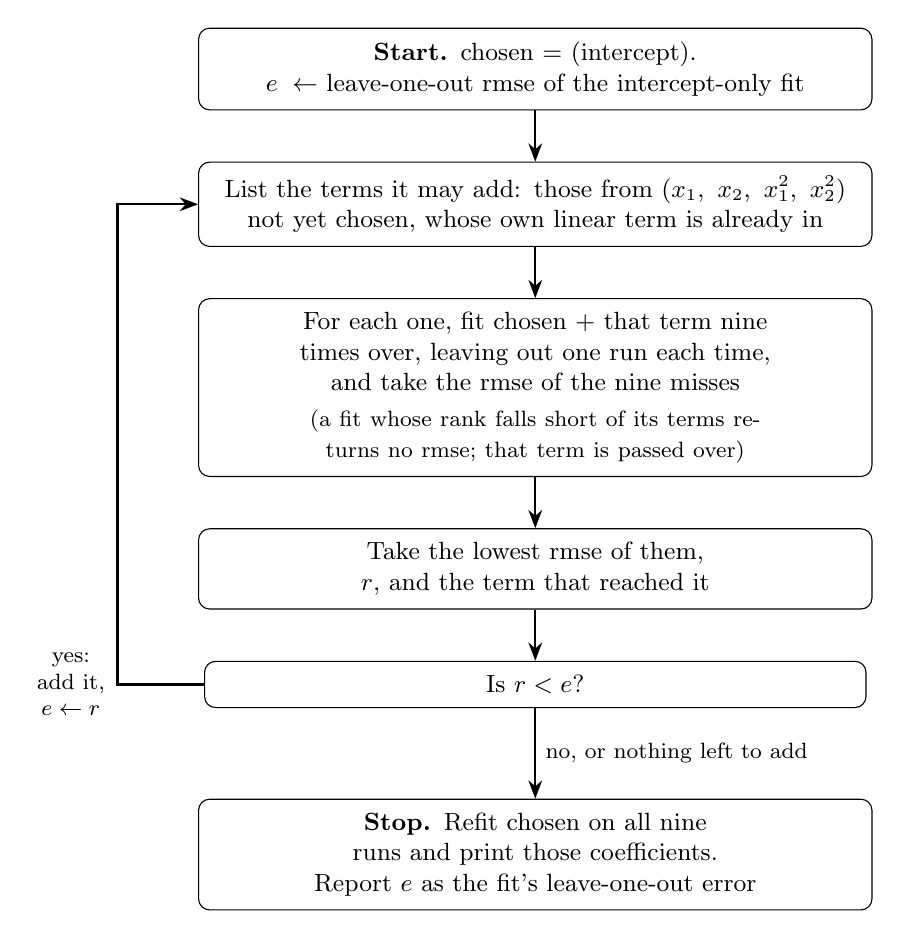
\begin{tikzpicture}[font=\small, node distance=0pt,
      box/.style={draw, rounded corners, align=center, inner sep=5pt, text width=8.2cm},
      arrow/.style={-Stealth, thick}]

    \node[box] (start) at (0,0)
      {\textbf{Start.} chosen $=$ (intercept).\\
       $e \leftarrow$ leave-one-out rmse of the intercept-only fit};

    \node[box, below=0.65cm of start] (allowed)
      {List the terms it may add: those from
       $(x_1,\; x_2,\; x_1^{2},\; x_2^{2})$ not yet chosen, whose own linear term is already in};

    \node[box, below=0.65cm of allowed] (score)
      {For each one, fit chosen $+$ that term nine times over, leaving out one run each time,
       and take the rmse of the nine misses\\[2pt]
       \footnotesize (a fit whose rank falls short of its terms returns no rmse; that term is
       passed over)};

    \node[box, below=0.65cm of score] (best)
      {Take the lowest rmse of them, $r$, and the term that reached it};

    \node[draw, rounded corners, below=0.65cm of best, inner sep=5pt,
          minimum width=8.4cm] (test)
      {Is $r < e$?};

    \node[box, below=1.15cm of test] (stop)
      {\textbf{Stop.} Refit chosen on all nine runs and print those coefficients.\\
       Report $e$ as the fit's leave-one-out error};

    \draw[arrow] (start) -- (allowed);
    \draw[arrow] (allowed) -- (score);
    \draw[arrow] (score) -- (best);
    \draw[arrow] (best) -- (test);
    \draw[arrow] (test) -- node[right, font=\footnotesize]
      {no, or nothing left to add} (stop);

    % the loop back up the left-hand side
    \coordinate (left) at ($(test.west) + (-1.1cm, 0)$);
    \draw[arrow] (test.west) -- (left) -- (left |- allowed.west) -- (allowed.west);
    \node[font=\footnotesize, align=center, left=1pt of left]
      {yes:\\ add it,\\ $e \leftarrow r$};
  \end{tikzpicture}
  \caption{Forward stepwise selection as \texttt{FittedOutcome.find\_best\_polynomial} runs it.
  The loop adds a term only when it lowers the leave-one-out error, so a term that merely fits
  the nine runs better never gets in.}
  \label{fig:stepwise}
\end{figure}

Run on recovery, the loop takes two steps and stops (Table~\ref{tab:stepwise-trace}). Current
density is offered at every step and rejected at every step: adding $x_1$ always makes the
out-of-sample error worse. Given that AN and AP disagree by $13.2$ points at the same current
density, that is the honest outcome.

\begin{table}[htbp]
  \centering
  \caption{The stepwise trace on recovery \%. Each cell is a full nine-fold leave-one-out rmse.
  Candidates are offered in the order $x_1$, $x_2$, $x_1^2$, $x_2^2$, so a tie goes to the
  simpler term.}
  \label{tab:stepwise-trace}
  \begin{tabular}{@{}llrl@{}}
    \toprule
    Step & Model so far & Its rmse & Terms offered, and their rmse \\
    \midrule
    0 & intercept                     & 15.052 & $x_1$: 16.244 \quad $x_2$: \textbf{7.898} \\
    1 & intercept, $x_2$              &  7.898 & $x_1$: 9.950 \quad $x_2^2$: \textbf{7.122} \\
    2 & intercept, $x_2$, $x_2^{2}$   &  7.122 & $x_1$: 9.471 --- nothing lower, stop \\
    \bottomrule
  \end{tabular}
\end{table}

That leaves~\eqref{eq:code-fit}, which the report prints as
\texttt{intercept +11.58,\allowbreak{} x2 -15.63,\allowbreak{} x2\_squared +6.08}. Its leave-one-out error is $7.122$
against the same bench scatter of $6.612$.

This is a far better equation than~\eqref{eq:five-term}: $7.122$ against $41.77$, and now
comfortably inside the $15.05$ of quoting the average, so it does carry real information about
the feed ratio. But $7.122$ is still larger than $6.612$, and that is the comparison that
decides. The fit misses a held-out run by more than the bench misses itself when it repeats a
setting, so nothing in the equation has been separated from the bench's own noise. The report
says so in those words --- \emph{worse than the bench repeating itself, so this fit has earned
no conclusion} --- and for the same reason the search under the gates returns no best setup: no
point inside the measured range clears the $35\,\%$ recovery floor.

\subsection{What would change the answer}

Two things would, and they are both runs rather than arithmetic.

Resolving AN against AP settles the yardstick. Those two are the same setting at
$25.67\unit{mA/cm^2}$ and $1.4277\unit{mol/mol}$ and they differ by $13.2$ points of recovery.
That single disagreement sets the $6.612$ that every fit is measured against, and until it is
either reproduced or explained, no fit can clear it. A third run at that setting either confirms
the spread, in which case recovery at high current density is genuinely that variable, or
identifies one of the two as faulty, in which case the scatter drops and $7.122$ may already be
good enough.

Runs off the cross make the interaction estimable and the curvature in $J$ real. A feed ratio
away from the lowest, at a current density away from the middle --- $R = 5.71$ at
$J = 25.67\unit{mA/cm^2}$, say --- breaks the identity
$(J - 13.6667)(R - 1.4277) = 0$, lifts the rank of the six-column design from $5$ to $6$, and
moves the support for the terms in $R$ off the three runs AF, AG and AT that currently carry
them alone.


\end{document}
